\documentclass[12pt]{article}

\usepackage{sbc-template}
\usepackage{graphicx,url}
\usepackage[brazil]{babel}
\usepackage[utf8]{inputenc}
\usepackage[T1]{fontenc}
\usepackage{enumitem}
\usepackage{placeins}
\usepackage{booktabs}

\graphicspath{{figuras/}}

\setlength{\textfloatsep}{5pt plus 2pt minus 2pt}
\setlength{\intextsep}{5pt plus 2pt minus 2pt}
\setlength{\floatsep}{5pt plus 2pt minus 2pt}
\setlength{\abovecaptionskip}{3pt}

\sloppy

\title{Avaliação de Branch Prediction em RISC-V no simulador gem5\\
Comparação entre LocalBP e BiModeBP e a sensibilidade ao padrão da carga}

\author{João Luís Almeida Santos\inst{1}}

\address{Bacharelado em Ciência da Computação\\
  Organização de Computadores
}

\begin{document}

\maketitle

\begin{resumo}
  Este trabalho avalia o impacto de dois preditores de desvios
  condicionais, o LocalBP, local e simples, e o BiModeBP, global e
  complexo, sobre uma carga rica em desvios, um simulador de combate de RPG
  que executa 1.000 partidas automáticas.
  O código assembly do primeiro trabalho foi adaptado para a sintaxe do GCC,
  compilado em um binário estático RISC-V e simulado no gem5 com uma CPU
  em-ordem. Do arquivo stats.txt foram extraídas a taxa de erro de predição,
  o IPC, o tempo de simulação e as operações descartadas. O BiModeBP reduziu
  a taxa de erro de 25,75\% para 21,86\%, aumentou o IPC em 1,8\% e descartou
  22\% menos operações. Um segundo experimento mostra que uma carga mais
  aleatória eleva o erro dos dois preditores, mas a vantagem relativa do
  BiModeBP se mantém.
\end{resumo}

\section{Introdução}

Preditores de desvio são peças centrais de processadores modernos. Em um
pipeline, cada desvio condicional mal previsto força o descarte de tudo o
que foi buscado especulativamente depois dele e custa uma penalidade de
vários ciclos \cite{hennessy2017quantitative}. O ganho de um preditor
depende do padrão de desvios da carga, foco deste trabalho.

Entre os temas propostos para o trabalho, este aborda o Tópico~2, sobre
branch prediction, e tem como objetivo comparar dois preditores condicionais
oferecidos pelo gem5 \cite{binkert2011gem5}, o LocalBP, local e simples, e o
BiModeBP, global e complexo. A carga usada é o
algoritmo do Trabalho~1, descrito na Seção~\ref{sec:jogo}. As métricas
são o total de desvios, os erros de predição, o IPC, o tempo de simulação e
as operações descartadas.

\section{O algoritmo avaliado}
\label{sec:jogo}

O algoritmo é um simulador de combate de RPG por turnos, escrito em RISC-V,
herdado do Trabalho~1. Dois jogadores se enfrentam e o programa joga 1.000
partidas automáticas, registrando o vencedor de cada uma pelo método de
Monte Carlo. A cada turno, o jogador da vez escolhe uma entre seis ações de
acordo com seus pontos de vida e de magia, o HP e o MP. A
Tabela~\ref{tab:skills} resume essas ações.

\begin{table}[ht]
\centering
\caption{Ações disponíveis a cada turno e seus efeitos.}
\label{tab:skills}
\small
\begin{tabular}{@{}llp{8cm}@{}}
\toprule
Habilidade & Custo & Efeito \\
\midrule
Atacar & livre & rola 1d20, 10 ou mais acerta e 20 dobra o dano \\
Defender & livre & bloqueia o dano, e rolagem alta gera contra-ataque \\
Soul Suck & livre & drena MP do inimigo e ganha quatro vezes para si \\
Absolute Grit & 20 MP & acerto crítico garantido, sem rolar o dado \\
Mirror Shield & 30 MP & reflete o próximo ataque recebido \\
Final Execution & 150 MP & 800\% de dano, falha se o alvo tiver mais de 50\% de HP \\
\bottomrule
\end{tabular}
\end{table}

O comportamento de cada jogador é definido por um bot, e o jogo tem três
deles, com lógicas distintas.

\begin{itemize}[nosep]
  \item Flowey sorteia a ação a cada turno, sem avaliar o estado do jogo.
  \item Chara segue um plano fixo. Acumula MP com Soul Suck, baixa o HP do
    inimigo abaixo de 50\% e encerra a partida com Final Execution.
  \item Toby reage à jogada do oponente, escolhendo a ação que tenta
    neutralizá-la.
\end{itemize}

A decisão de cada bot depende de comparações sobre HP e MP, que o compilador
traduz em desvios condicionais, de modo que prever o salto equivale a prever
a jogada do bot. Isso torna o algoritmo adequado para avaliar preditores.

\section{Fundamentação Teórica}

Um desvio condicional é um ponto do programa em que a execução pode seguir
dois caminhos. Quando a condição se cumpre, o desvio é tomado e a execução
salta para outro endereço; quando não se cumpre, o desvio não é tomado e a
execução segue para a instrução seguinte. O processador precisa escolher o
caminho antes de a condição ser calculada, para não parar o pipeline. Essa
escolha é o palpite do preditor, e um palpite errado joga fora o trabalho já
adiantado e custa ciclos.

\subsection{Preditor local}

O palpite vem de um contador de 2 bits que mede a confiança no caminho, com
quatro níveis que vão do não-tomado forte ao tomado forte. Cada vez que o
desvio é tomado o contador sobe um nível, e quando não é tomado ele desce. O
palpite é tomado nos dois níveis de cima e não-tomado nos dois de baixo.
Como é preciso mover dois níveis para trocar de lado, um resultado fora do
padrão não inverte o palpite na hora. Um laço que quase sempre repete, por
exemplo, segue previsto como tomado até a iteração em que enfim termina.

O LocalBP \cite{smith1981branch} guarda um contador desses para cada desvio,
escolhido pelo PC, o endereço do desvio na memória, de modo que cada desvio
aprende a própria tendência. É simples e barato, mas não relaciona um desvio
com outro e, como a tabela tem tamanho fixo, dois desvios podem disputar o
mesmo contador e se atrapalhar.

\subsection{Preditor global bimodal}

O histórico global é um registro dos resultados dos últimos desvios do
programa, e permite capturar padrões repetidos. O BiModeBP
\cite{lee1997bimode} indexa suas tabelas combinando esse histórico com o PC e
mantém duas tabelas de contadores, uma para os desvios que costumam ser
tomados e outra para os que costumam não ser, mais uma tabela que escolhe
entre elas. Essa separação reduz a interferência que prejudica o LocalBP, ao
custo de mais área e complexidade.

\section{Metodologia}

\subsection{Adaptação e configuração}

O código original main.s usa as chamadas de sistema do RARS. Para o gem5,
ele foi adaptado em main\_gem5.s, com as diretivas e o ponto de entrada
\_start na sintaxe do GCC, e compilado como binário estático com
{\ttfamily\small riscv64-linux-gnu-gcc -nostdlib -static main\_gem5.s -o
output/main\_gem5}. A configuração veio de um script Python fornecido pelo
professor, ajustado para usar o modelo de CPU em-ordem MinorCPU, como pede o
Tópico~2, e no qual só o preditor condicional muda entre as rodadas, de
LocalBP para BiModeBP. Como só o preditor muda, a comparação é justa. A seed
do jogo vem do relógio, então as contagens absolutas mudam um pouco a cada
execução e a análise usa taxas, que são estáveis.

\subsection{Duas cargas de trabalho}
\label{sec:cargas}

Um preditor só tem ganho quando há regularidade a explorar. Para medir esse
efeito foram montadas duas cargas com graus diferentes de previsibilidade,
variando apenas o bot atribuído aos jogadores.

\begin{itemize}[nosep]
  \item Carga mista (main\_gem5.s). O bot de cada jogador é sorteado a cada
    partida, misturando comportamento determinístico e aleatório, o que
    produz uma carga parcialmente previsível.
  \item Carga aleatória (main\_gem5\_random.s). Os dois jogadores ficam
    fixos no Flowey, de modo que toda escolha de ação é um sorteio. Essa
    variante foi gerada a partir do código original, alterando somente a
    atribuição de bot no \_start.
\end{itemize}

Cada carga foi simulada com os dois preditores, totalizando quatro execuções
de 1.000 partidas cada.

\section{Resultados}

A Tabela~\ref{tab:metricas} reúne as métricas da carga mista. A taxa de erro
de predição é a razão condIncorrect / condPredicted.

\begin{table}[ht]
\centering
\caption{Métricas da carga mista no MinorCPU, extraídas do stats.txt.}
\label{tab:metricas}
\begin{tabular}{lrr}
\toprule
Métrica & LocalBP & BiModeBP \\
\midrule
Desvios condicionais avaliados & 606.368 & 575.382 \\
Desvios condicionais incorretos & 156.136 & 125.793 \\
Taxa de erro de predição & 25,75\% & 21,86\% \\
IPC & 0,7731 & 0,7868 \\
Tempo simulado & 13,969\,ms & 13,808\,ms \\
Instruções efetivadas & 10.799.891 & 10.864.867 \\
Operações descartadas & 309.544 & 242.246 \\
\bottomrule
\end{tabular}
\end{table}

\subsection{Carga mista}

Os resultados estão na Tabela~\ref{tab:metricas}. O BiModeBP errou 21,86\%
dos desvios condicionais contra 25,75\% do LocalBP, uma redução relativa de
15\%. Menos erros significam menos descartes, então o IPC subiu de 0,7731
para 0,7868, mais 1,8\%, e o tempo caiu 1,2\%. O BiModeBP também descartou
242 mil operações contra 310 mil do LocalBP, 22\% a menos.

\subsection{Sensibilidade ao padrão de desvios da carga}
\label{sec:sensibilidade}

O experimento foi repetido na carga aleatória da Seção~\ref{sec:cargas}, com
dois efeitos visíveis na Figura~\ref{fig:wlmis}. Os dois preditores pioram,
com a taxa de erro subindo de 25,75\% para 30,22\% no LocalBP e de 21,86\%
para 25,65\% no BiModeBP, pois sortear a ação remove o viés dos desvios e um
desvio sem viés é imprevisível por construção. A vantagem relativa do
BiModeBP, porém, fica em torno de 15\% nas duas cargas, então a carga
aleatória é mais difícil para ambos sem anular o ganho do preditor global.

\begin{figure}[ht]
\centering
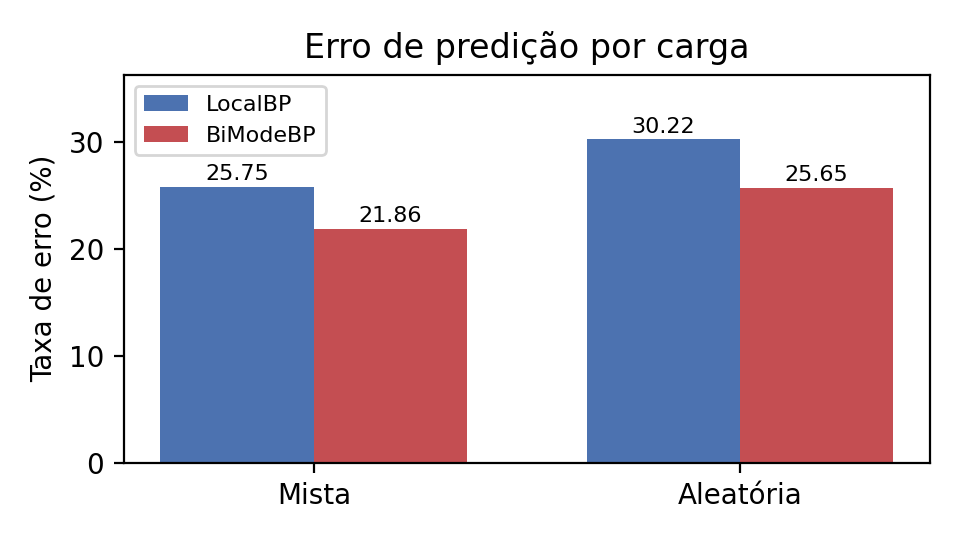
\includegraphics[width=0.36\textwidth]{wl_mispred.png}
\caption{Taxa de erro de cada preditor nas cargas mista e aleatória.}
\label{fig:wlmis}
\end{figure}

\FloatBarrier

\section{Discussão}

Para esta carga o BiModeBP é o preditor mais adequado, e a razão está na
lógica dos bots. A Chara repete o mesmo plano em todas as partidas, usando
Soul Suck até juntar MP e disparando o Final Execution em seguida. Isso gera,
partida após partida, a mesma sequência de comparações sobre MP e HP, um
padrão repetido que o histórico global do BiModeBP aprende e que o LocalBP,
preso a cada desvio isolado, não captura. O Flowey, ao sortear a ação,
produz desvios sem padrão, que nenhum preditor acerta acima do acaso.

O aumento de 1,8\% no IPC é modesto porque parte das decisões do jogo não
tem viés e não pode ser prevista. O BiModeBP extrai ganho apenas da parcela
previsível, ao custo de um hardware mais complexo.

\section{Conclusão}

O LocalBP e o BiModeBP foram comparados sobre o mesmo binário RISC-V no
gem5. O BiModeBP venceu em todas as métricas e confirma a teoria, já que
cargas com desvios correlacionados, como os planos repetidos dos bots, se
beneficiam de um preditor com histórico global.

O segundo experimento qualifica essa conclusão. Ao tornar as decisões
puramente aleatórias, os dois preditores erram mais, mas a vantagem relativa
do BiModeBP se mantém em torno de 15\%.

\bibliographystyle{sbc}
\bibliography{referencias}

\end{document}
